\chapter{Medical background}
\label{chapter:medical_background}

\section{Human teeth}
Human dentition is composed of two sets of teeth - primary and permanent. The primary, also called deciduous, consists of 20 teeth and begins to erupt at six months of age. This dentition is completely replaced at the approximate age of 13 years by a permanent set of teeth, including 32 teeth. These can be divided into four classes based on function and form. Namely, those classes are:

\subsubsection*{Incisors}
A total of 8 incisors teeth are found in primary and permanent dentition. They are located at the oral cavity entrance, and their primary purpose is to cut and shear food. They are essential for a smile's esthetics and play a vital role in phonetics.

\subsubsection*{Canines}
A total number of four canines are located at the corners of dental arches, dividing them into a frontal and a lateral part. They have a triangular shape with a single cusp tip on the incisal edge. The structure is associated with their ability to seize, pierce, tear and cut food. Along with the incisors, they are essential for esthetics.

\subsubsection*{Premolars}
Premolars are teeth found only in permanent dentition, being the successional teeth of all primary eight molars. Premolars share functional characteristics of canines and molars - they both seize and grind food thanks to their anatomy.

\subsubsection*{Molars}
Human dentition contains 12 permanent molars with no deciduous predecessors. Their leading role is crushing and grinding food to dimensions appropriate for swallowing. Broad occlusal surfaces make them capable of this task. Molars are prone to dental caries due to deep grooves that run across the occlusal surface of the teeth and a vast area of contact between adjacent molars. Both of these places are difficult to clean, resulting in a space where bacterias tend to accumulate.


\subsection{Structure of teeth}
Teeth are composed of three structures: Enamel, pulp-dentin complex, and cementum. A picture of teeth structure is depicted in the figure

    *{Enamel}
The superficial layer covering the anatomic crown of a tooth consists of a highly mineralized crystalline structure called the enamel. More than 90\% of the volume is taken up by minerals (hydroxyapatite), making enamel the hardest substance of teeth and even the human body. Its thickness varies from one class of tooth to another, but it ranges from 2 to 3mm on average. Enamel is produced in the process of amelogenesis by cells occurring only in the development stage, meaning that it cannot regenerate. The biggest threat to enamel are acidic conditions, which can cause its demineralization. Enamel has the ability to remineralize, but if the cause is not removed, the enamel is irreversibly damaged, and a cavity is formed.

\subsection*{Pulp-Dentin complex}
Pulp and dentin are two specialized connective tissues. However, some sources consider them a single tissue forming a complex \cite{2019a}.
The dental pulp is located in the pulp chamber of the tooth, and it serves four functions: formative, nutritive, sensory, and reparative.
The pulp is circumscribed by dentin formed by specific cells in the process of dentinogenesis. Their cell bodies are found in the pulp chamber, but their cytoplasmic cell processes, located in dentinal tubules, extend into the mineralized dentin. Thanks to those processes, dentin is considered to be living tissue. Its function is to provide the ability to regenerate and react to pathological stimuli, such as blocking the advancement of carious lesions by precipitating minerals in the affected area.
Dentin forms the most significant portion of the tooth. In the coronal part, it is covered by the enamel, and on the anatomic root of the tooth overlayed by cementum. There are different types of dentin.
\begin{itemize}
    \item \textbf{Primary dentin} forms the outer and most prominent layer of dentin closest to the enamel. It is produced in the development stage of the tooth.
    \item \textbf {Secondary dentin} is formed after the root development is completed.
    \item \textbf{Tertiary reactive dentin} production is encouraged as a response to pathological stimuli, such as injury or caries. It is produced at the pulp-dentin interface in order to protect the pulp.
    \item \textbf{Transparent dentin} is characterized by the presence of mineral precipitates in dentinal tubules as a result of injury or aging.
\end{itemize}


\subsection*{Cementum}
Cementum covers the anatomic roots of teeth. Its structure consists of approximately 50 \% of anorganic material, 50 \% of organic matter, and water, making it slightly softer than dentin and far more delicate than enamel. Together with gingiva, periodontal ligaments, and the alveolar bone, cementum forms periodontium, ensuring that the tooth is attached to the bone. Cementum possesses the ability to repair itself to a limited degree.

\section{Dental caries}

\subsection{Cause}
Dental caries is an infectious disease characterized by the demineralization of hard dental tissues. The leading cause is dental plaque (also called a biofilm). Plaque is composed of bacteria, their by-products, and saliva, and it has the ability to adhere to the tooth structure. Some bacteria in the plaque metabolize refined dietary carbohydrates and produce organic acid by-products. If present in the biofilm for an extended period of time, those acids can lower the PH in the biofilm to below a critical threshold (5.5 for enamel, 6.2 for dentin)\cite{2019a}. Low pH drives phosphate and calcium from the tooth into the biofilm in an attempt to reach an equilibrium. This loss of minerals in a tooth is called demineralization and, if not stopped, can lead to a caries lesion. However, this process can be controlled and eventually reverted if the pH returns to neutral and the relative concentration of soluble calcium and phosphate in the biofilm is higher than in the tooth. This process occurs multiple times a day and is modulated by many highly individual and tooth-specific factors. They will differ from person to person.


\subsection{Classification of dental caries}
\label{sec:caries_classification}
Dental caries are classified on multiple bases. The common ones are the depth of the lesion or lesion activity. \newline
A frequently used classification scheme was proposed by Pitts \& Fyffe in 1988 \cite{2019a}, including a total of 4 categories, three for cavitated lesions and one for non-cavitated lesions.
\begin{itemize}
    \item \textbf{D0} Surface sound. No evidence of either treated or untreated caries.
    \item \textbf{D1} Initial Caries. No detectable loss of tooth substance. Staining in fissures or rough spots in enamel may be visible, but these spots do not catch the explorer.
    \item \textbf{D2} Enamel caries. Demonstrable loss of tooth substance. The chalky or crumbled texture of the material within the cavity. No evidence that cavitation has penetrated through the enamel layer into the dentin.
    \item \textbf{D3} Caries of dentin. The floor or wall of the cavity is softened. The tip of the explorer must enter a lesion with certainty.
    \item \textbf{D4} Pulpal involvement. Deep cavity with probable involvement of the pulp. A probe should not be used to probe the pulp.
\end{itemize}

\subsection{Diagnosis}
Visual-tactile diagnosis is the primary way to inspect teeth and detect caries. Dentists use a mouth mirror and sharp probe to perform the examination. It is vital to dry teeth since the difference in the refractive index between sound and carious enamel is higher when water is removed from the tissue. This increases the chance of spotting a carious lesion before it has an opportunity to progress and cavitate the tooth.
The second most used method clinicians use to complement the visual examination is a dental X-ray. In dentistry, there are two main types of X-ray imaging taken during the examination: intraoral (the X-ray film is located inside the mouth) and extraoral (the X-ray film is outside the mouth). The intraoral images are the most commonly taken ones. This category includes bitewing and periapical X-rays, each featuring different aspects of the teeth. Extraoral imaging is mainly used to detect dental problems in the jaw and skull area. The most common one to be used is a panoramic radiograph \cite{2015}. \newline
Less common diagnostic measures are:

\begin{itemize}
    \item Laser light-induced fluorescence
    \item Digital imaging fiber-optic transillumination
    \item Electrical conductance and impedance measurement
\end{itemize}

\subsubsection{Bitewing X-ray}
The bitewing radiograph is an image that depicts the upper and lower teeth in one region of the mouth, as seen in figure \ref{fig:bitewing_sample}. It gives a clear sight of the interproximal surfaces allowing good caries detection in this area. Interproximal caries are challenging to diagnose by the visual-tactile method; thus, using the bitewing X-ray can lead to an early diagnosis and a chance for the enamel to remineralize. Also, it portrays the alveolar crest, where the dentist may notice any bone thickness changes due to periodontal disease. Unlike the other intraoral method, it does not show the entire length of the teeth. This type of dental X-ray is the most commonly taken for preventive purposes \cite{2015}.

\begin{figure}
    \begin{floatrow}[2]
        \ffigbox[\FBwidth]{\caption{Bitewing X-ray image}\label{fig:bitewing_sample}}%
        {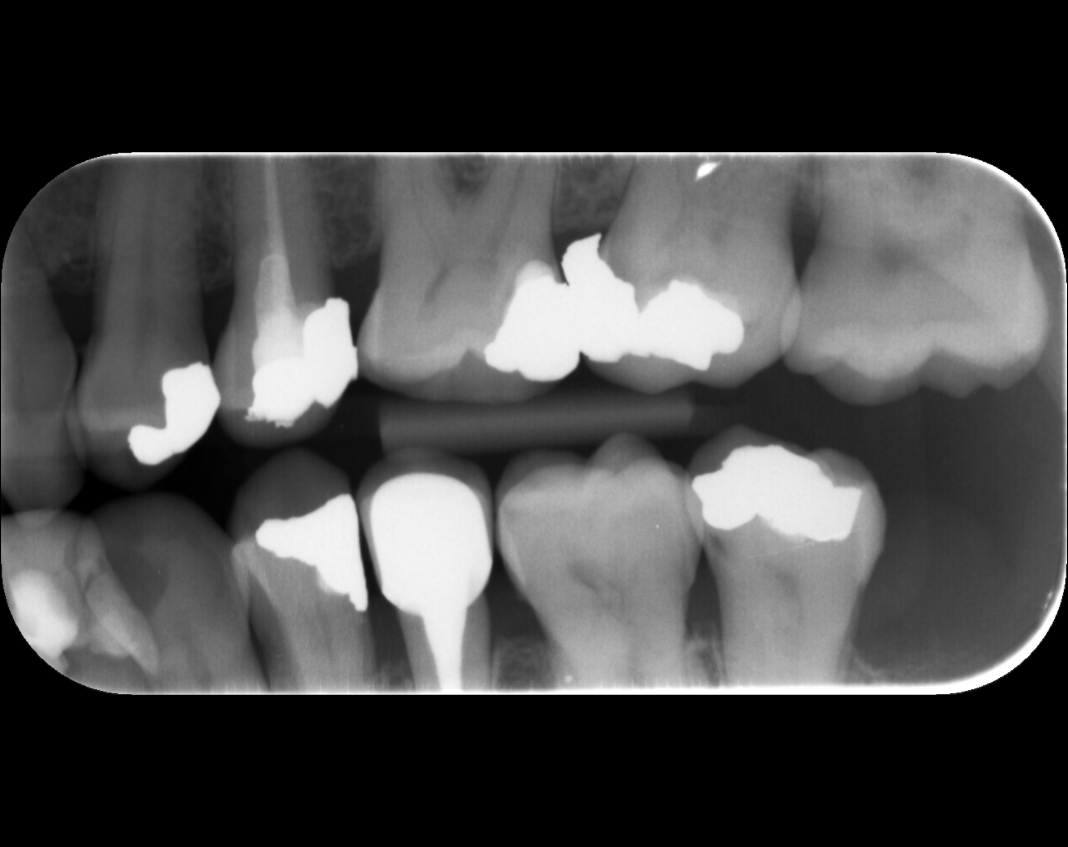
\includegraphics[width=\linewidth]{images/bitewing_xray.png}}\;
        \ffigbox[\FBwidth]{\caption{Periapical X-ray image, source \cite{Creanga2015}}\label{fig:periapical_sample}}%
        {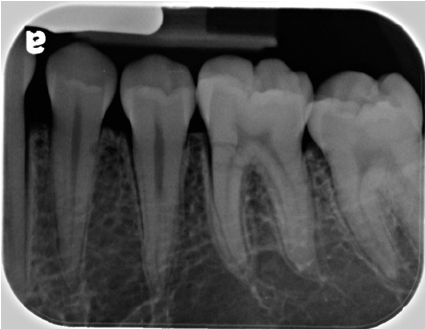
\includegraphics[width=\linewidth]{images/periapical_xray.png}}
    \end{floatrow}
\end{figure}

\subsubsection{Periapical X-ray}
Periapical X-ray portrays the tooth from the crown to where the root attaches to the jaw; hence, the whole tooth length is visible. As illustrated in the figure\ref{fig:periapical_sample}, it only shows the upper or lower teeth in one part of the jaw.  Periapical X-ray detects any abnormalities in the root and any periapical lesions.

\subsubsection{Panoramic X-ray}
This extraoral dental image shows the entire mouth area, including the upper and lower jaw and adjacent structures. It depicts the fully emerged teeth and the ones that are not fully erupted yet. Impacted teeth, i.e. wisdom teeth as seen in the figure, can be identified \ref{fig:panoramatic_xray}as well. Panoramic X-ray is often used before major procedures or to diagnose jaw tumors, cysts, fractures, or sinusitis. Nevertheless, it is not usually taken to diagnose dental caries \cite{clevland_xray}.

\begin{figure}
    \centering
    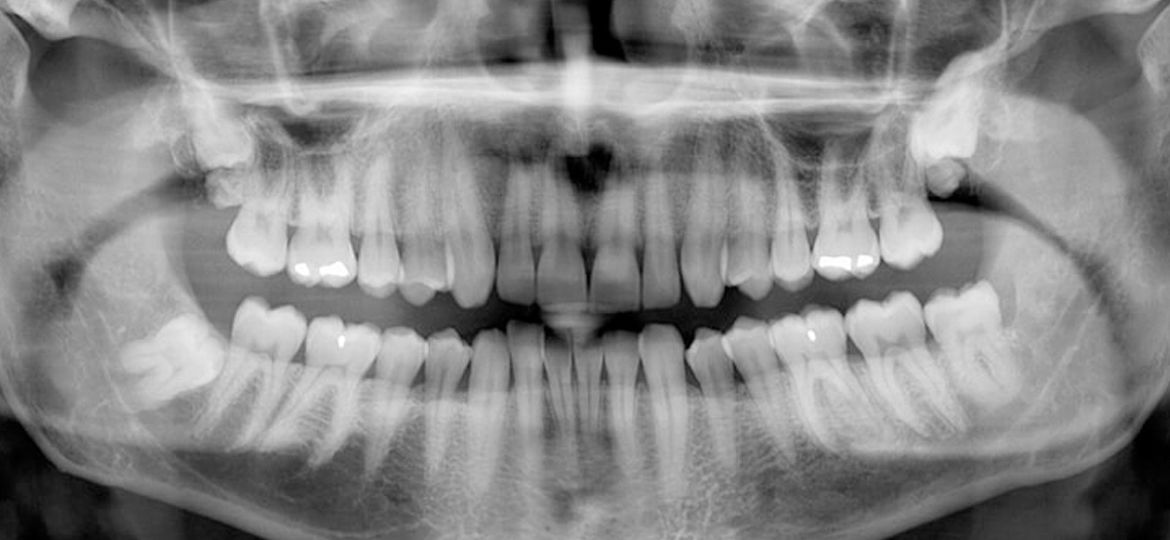
\includegraphics[width=\linewidth]{images/panoramatic_xray.jpg}
    \caption{Panoramic X-ray image, source \cite{Panoramatic2017}}
    \label{fig:panoramatic_xray}
\end{figure}


\subsubsection{Digital imaging fiber-optic transillumination (DIFOTI)}
DIFOTI is different from the previously mentioned types of dental imaging. It works with infrared fiber-optic light and not an X-ray, unlike the others. A lesion's optical properties differ from those in healthy dental tissue, making it appear darker. DIFOTI enables the detection of fissure/occlusal caries, interproximal caries, and fractures and cracks in the tooth. It is a noninvasive method since it does not expose the patient to ionizing radiation \cite{Strassler2014}.

\subsection{Treatment}
Treatment is suggested based on the progression of the lesion and the patient's risk profile. In some cases, only instructions to increase oral hygiene together with fluoride toothpaste are enough to stop the progression and lead to remineralization of the enamel. The dentist can suggest an application of a sealant to prevent further progression of the lesion. If this treatment is perceived as insufficient given the mentioned factors, restoring the tooth is required. This consists of removing all dental decay and filling the cavity with restorative material such as dental composite or amalgam \cite{2019a}\cite{2015}.

\subsection{Epidemiology}
Untreated dental caries in permanent teeth is the most prevalent medical condition \cite{Kassebaum2015}. In 2010 around 35\% of the global population was affected. The most considerable prevalence was observed around the age of 25. The sex of a person was not a significant factor in the statistics. No noticeable change in prevalence occurred between 1990 and 2010 \cite{Kassebaum2015} \cite{Frencken2017}, which means that the technological improvement in dentistry did not affect the prevalence.
Kassebaumet al. suggest that 42 new cases of tooth decay in primary and permanent teeth will develop annually from observing 100 people. This imposes a burden on health care systems. According to Huang et al., \cite{Hung2020} in the United States alone, the cost of dental care in 2016 was 0.1 trillion \$ out of total health care expenditure of 1.62 trillion \$.

,